\chapter{Transport Layer Security}
TLS, or Transport Layer Security, was originally proposed by Netscape
in 1995 as a way to secure communications between a web browser and a
web server. It is the successor to SSL, or Secure Sockets Layer, which
was first introduced by Netscape in 1995. The two terms are often used
interchangeably, but TLS is the more modern and secure protocol.\\ 
The main goal of SSL was to create secure network channel, almost at
session level(4.5), between two parties, to provide some security
services that neither TCP nor IP provides:
\begin{itemize}
  \item \textbf{peer authentication} based on asymmetric
    challenge-response authentication(the challenge for the service is
    implicit, while for the client is explicit). Server authentication
    is alway compulsory, while client authentication is optional and
    requested by the server.
  \item \textbf{message confidentiality} base on symmetric encryption
  \item \textbf{message integrity} and authentication based on MAC
    computed on the trasmitted data
  \item \textbf{replay, filtering and reordering attack protection}
    using implicit record numbers( the correct order of transmission
    is provided by TCP, for this reason the number is implicit). This
    number is used also in the MAC computation.

\end{itemize}

You can see the TLS packet structure in figure
\ref{fig:tls-packet-structure}.
The TLS handshake protocol is used to establish a new session or 
reestablish an existing session. The TLS change cipher spec protocol 
is used to trigger the change of the algorithms to be used for message 
protection, or most notably to pass from the previous unprotected 
session to a protected one. The TLS alert protocol is used to signal
errors or signal the end of the connection. 
The TLS record protocol contains the generic protocols informations
and its content depend of the state of the connection and the protocol
it is tunneling.
\begin{figure}[H]
    \centering
    \includegraphics[width=.6\textwidth]{img/TLS packet
    structure.png}
    \caption{TLS packet structure.}
    \label{fig:tls-packet-structure}
\end{figure}

\section{TLS session and connection}
It is important to make a clear distinction between TLS session and
connections.\\
\textbf{TLS sessions} a \textbf{logical association} between client and server, created
via an handshake protocol and its shared between different TLS
connections(1:N).\\
\textbf{TLS connections} are a \textbf{transient TLS channel} between client and server,
which means that each connection is associated with only one specific
TLS session(1:1).

\begin{figure}[H]
  \centering
  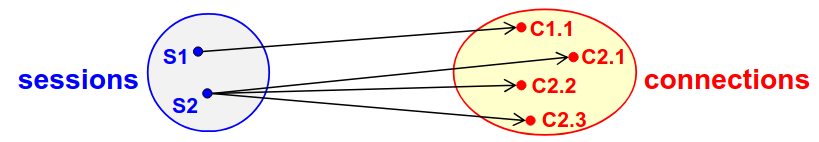
\includegraphics[width=.7\textwidth]{img/TLS session connection.png}
  \caption{TLS session and connection.}
  \label{fig:tls-session-and-connection}
\end{figure}
\section{TLS handshake protocol}
The TLS handshake protocol is used to establish a new session or
reestablish an existing session. It's a critical part of the TLS
protocol, because the channel pass from an unprotected state to a
protected one. During this phase the two parts agree
agree on a set of algorithms for confidentiality and integrity,
exchange random numbers between the client and the server to be used
for the subsequent generation of the keys, establish a symmetric key
by means of public key operations (originally RSA and DHKE, but
nowadays the elliptic curve versions of algorithms are used) and negotiate the
session-id and exchange the necessary public keys certificates for the
asymmetric challenge-response authentication.

\section{Achieving Data protection}
Data protection is achieved by using symmetric encryption algorithms
to encrypt the data and Message Authentication Codes(MAC) to ensure
the integrity of the data and the authentication of the sender.\\
Figure \ref{fig:tls-data-protection} shows how the data protection is 
achived in TLS using authenticate-then-encrypt approachm, but also
encrypt-then-authenticate is possible.\\
The MAC is computed over the data(compressed or not), the TLS sequence 
number and the key used for the MAC computation. The padding is also
part of the MAC computation to avoid those attacks that change the
padding.\\
The MAC is then encrypted with the dedicated symmetric key and a
suitable initialization vector(IV) 

\begin{figure}[H]
  \centering
  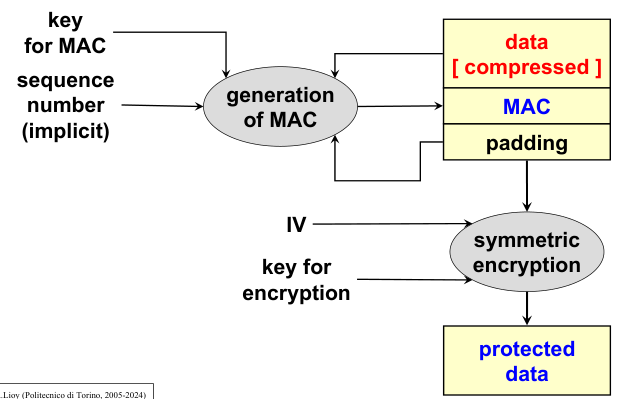
\includegraphics[width=.5\textwidth]{img/TLS data protection.png}
  \caption{TLS data protection.}
  \label{fig:tls-data-protection}
\end{figure}

The keys are \textbf{directional}, so there are two keys( one for
client to server and one for server to client) to protect against
reuse of the sequence number in the opposite direction.

\section{Relationship among keys and sessions}
When a new session is created using the handshake protocol, a new
\textbf{pre-master secret} is established using public key
cryptography. Then from the session a new connection is created, which
requires a random number to be generated, and exchanged between the
client and the server. Those two values are combined via a KDF,
usually HHKDF( HMAC-based key derivation function) to generate the 
\textbf{master secret}. This computation is done only once, and the 
secret is common to several connections.\\
The pre-master secret is then discarded, and the keys necessary for
the MAC computation, encryption and, if necessary, IVs will be derived
from the master secret.\\
You can notice that the master secret is common to any connections
inside a session, but the per-connection keys are different every
time. This is another important feature to avoid replay attacks,
possible because numbering is per-connection. This solution also
allows to reduce the cost of establishing new keys for each
connection.

\begin{figure}[H]
  \centering
  \includegraphics[width=.5\textwidth]{img/relationship
  keys-connection.png}
  \caption{Relationship among keys and sessions.}
  \label{fig:tls-keys-and-sessions}
\end{figure}

\section{Perfect Forward Secrecy}
Since the keys are generated from symmetric crypto, if the private key
used to perform encryption and decryption of the pre-master secret is
compromised, all the previous communication can be decrypted because
it is possible to derive the master-secret. This is only possible if
the server has a certificate valid for both signature and encryption
In this context, perfect forward secrecy is desirable.
\begin{boxH}
  \textbf{Perfect Forward Secrecy} is a property of key-agreement
  protocols ensuring that the compromise of the secret key used for 
  will compromise only current (and eventually future) traffic but not
  the past one
\end{boxH}
The most common way to achieve this is to use \textbf{ephemeral keys},
which are one-time asymmetric keys( used for key exchange). This means
that the key pair used for key exchange is not a long term key pair,
but a temporary one generated on-the-fly when necessary.\\ 
The ephemeral key needs to be authenticated, so only for this purpose
the long-term key is used for signing the ephemeral key. This is done
using DHKE instead of RSA because the latter one is really slow, while
the former one is faster with the compromise of only using the
established key for a certain number of session.\\
Let's now go over some considerations: if the temporary key is
compromised, perfect forward secrecy of the communication is still
valid because he can only decrypt the traffic exchanged using the
temporary key. On the contrary, if the long-term key is compromised,
no secret is really disclosed, because no traffic has been exchanged
using it for encryption, but is still a problem for server
authentication.

\section{The protocol}
The TLS handshake is always initiated by the client. 

\subsection{Client Hello and Server Hello}
In version 1.2 the client sends a \textbf{Client Hello}, which
contains:
\begin{itemize}
  \item the SSL version preferred by the client, and the highest
    supported(2=SSL-2, 3.0=SSL-3, 3.1=TLS-1.0, \dots)
  \item a 28 bytes pseudo-random number, which is the client random
  \item a session-id, which is \textit{0} if the client is starting a
    new session, and \textit{1} if the client is trying to resume a
    previous session
  \item a list of cipher suites supported by the client, in order to 
    let the server choose the most secure one (the set of algorithms
    used for encryption, for key exchange, and for integrity)
  \item a list of compression methods supported by the client
    (supported only up to TLS 1.2)
\end{itemize}

And then a \textbf{server hello} is sent back, which contains:
\begin{itemize}
  \item the SSL version chosen by the server, the highest one
    supported by both the client and the server
  \item a 28 bytes pseudo-random number, which is the server random
  \item a session identifier(session-id), which is a new one if the
    server is starting a new session, and the same as the client's if
    the server is resuming a previous session
  \item the cipher suite chosen by the server, the strongest common
    one between the client and the server
  \item the compression method chosen by the server
\end{itemize}


\begin{figure}[H]
  \centering
  \begin{subfigure}{.5\textwidth}
    \centering
    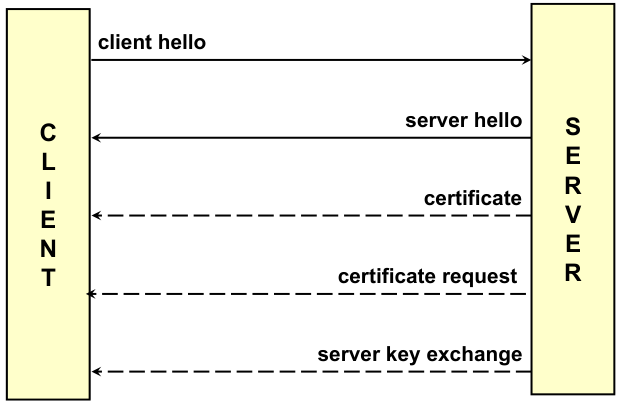
\includegraphics[width=.9\linewidth]{img/TLS key echange.png}
    \caption{The TLS handshake protocol(TLS 1.2).}
    \label{fig:tls-handshake-protocol-1.2}
  \end{subfigure}%
  \begin{subfigure}{.5\textwidth}
    \centering
    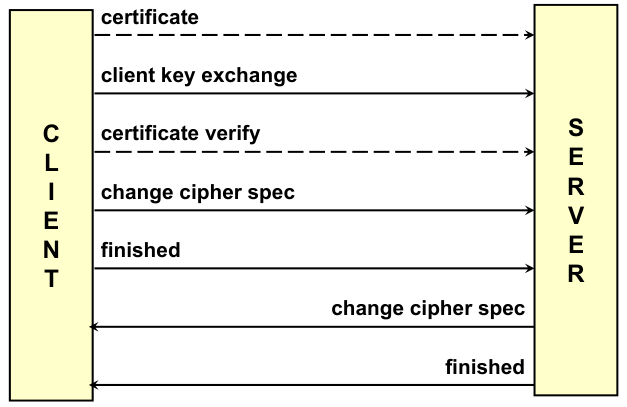
\includegraphics[width=.9\linewidth]{img/TLS key exchange 1-3.png}
    \caption{The TLS handshake protocol(TLS 1.3).}
    \label{fig:tls-handshake-protocol-1.3}
  \end{subfigure}
\end{figure}

\subsection{Cipher suite}
A cipher suite is a string which contains the set of cryptographic
algorithms used in the TLS protocol. A typical cipher suite consists
of a key exchange algorithm, the symmetric encryption algorithm, and
the hash function used for generating MACs.
Some example of those are:
\begin{itemize}
  \item SSL\_NULL\_WITH\_NULL\_NULL (no protection, used for the record
    protocol to be used in the handshake)
  \item SSL\_RSA\_WITH\_NULL\_SHA
  \item SSL\_RSA\_EXPORT\_WITH\_RC2\_CBC\_40\_MD5
  \item SSL\_RSA\_WITH\_3DES\_EDE\_CBC\_SHA
\end{itemize}


\subsection{Certificates}
After the initial exchange, the server is ready to authenticate
itself.\\
The server sends its long-term public key certificate to the client
for server authentication. Actually, the whole certificate chain, up
to the root CA, must be sent. Furthermore , the subject of the 
certificate must match the server name.\\
Server authentication is implicit, because its private key is used to
decrypt the pre-master secret, while client authentication is 
always explicit.

\begin{boxH}
  The implicit server authentication is based on the fact that the MAC
  is computed trough the key derived trough knowledge of the private
  key, so only the server can compute it.
\end{boxH}

Optionally, the server can request a certificate from the client for
client authentication. In this case the server specifies the list of
trusted CA's, and the client sends its certificate chain. The browsers
show to the users (for a connection) only the certificates issued by
trusted CAs.
If client certificate verification is required, an explicit request to
send the hash computed over all the handshake messages before this 
one and encrypted with the client private key is sent to the client.

\subsection{Key exchange}
The key exchange is the most important part of the handshake protocol.
If the server is using RSA for key exchange, the client generates a
pre-master secret, encrypts it with the server's public key(which can
be ephemeral or from its x.509 certificate) and sends it to the
server. If RSA is no used, DHKE can be used to generate the pre-master
secret, and in this case the server computes the value independently 
and the two parts can derive the master secret.\\
Another option is to use FORTEZZA, which is a key exchange algorithm
based on DH.

\subsection{Certificate verify}
In case the server requested client authentication, the client will be
required to send the certificate to prove that he is the owner of it's
private key. The message to be signed is the hash of all the messages
exchanged up to this point in the handshake protocol. This is to avoid
replay attacks too.


\subsection{Change cipher spec}
The change cipher spec message used to trigger the change of the
algorithms to be used for message protection. It allows to pass from
the previous unprotected messages to the protection of the next
messages with algorithms and keys just negotiated, thus is technically
a protocol on its own and not part of the handshake. Some analysis
even say that it could be removed from it.


\subsection{Finished message}
The finished message is the last message of the handshake protocol,
and the first message protected by the negotiated keys and algorithms.
It is necessary to ensure that the handshake has not been tampered
with, and it contains contains a MAC computed over all the previous
handshake messages (but change cipher spec) using as a key the master
secret. Notice that the finished message is different for the client 
and the server, because the MAC is computed over different messages.

This allows to prevent rollback man-in-the-middle attacks (version
downgrade or ciphersuite downgrade)

% 3 subfig, 2 on top and 1 on bottom
\begin{figure}[H]
  \centering
  \begin{subfigure}{.5\textwidth}
    \centering
    \includegraphics[width=.9\linewidth]{img/TLS no ephimeral no
    auth.png}
    \caption{TLS handshake(no ephemeral, no client authN).}
    \label{fig:tls-handshake-protocol}
  \end{subfigure}%
  \begin{subfigure}{.5\textwidth}
    \centering
    \includegraphics[width=.9\linewidth]{img/TLS no ephimeral
    auth.png}
    \caption{TLS handshake(no ephemeral, client authN).}
    \label{fig:tls-handshake-protocol-2}
  \end{subfigure}
  \begin{subfigure}{.5\textwidth}
    \centering
    \includegraphics[width=.9\linewidth]{img/TLS ephimeral no
    auth.png}
    \caption{TLS handshake(ephemeral, no client authN).}
    \label{fig:tls-handshake-protocol-3}
  \end{subfigure}
  \caption{TLS handshake protocol.}
\end{figure}

\section{Setup Time}
The setup time is the time required to establish a secure connection 
between the client and the server. TLS depends on TCP, so the TCP
handshake must be taken into account. Then the TLS handshake is
performed, meaning that typically 3 RTTs (1 for TCP and 2 for TLS) are
required to establish a secure connection. Usually after 180ms the two
parties are ready to send protected data( assuming 30ms delay
one-way).

% 2 subfig
\begin{figure}[H]
  \centering
  \begin{subfigure}{.5\textwidth}
    \centering
    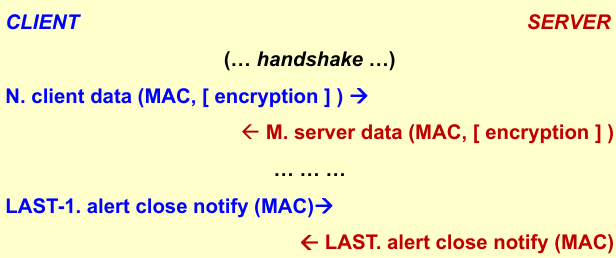
\includegraphics[width=.9\linewidth]{img/TLS link teardown.png}
    \caption{TLS link teardown.}  
    \label{fig:tls-link-teardown}
  \end{subfigure}%
  \begin{subfigure}{.5\textwidth}
    \centering
    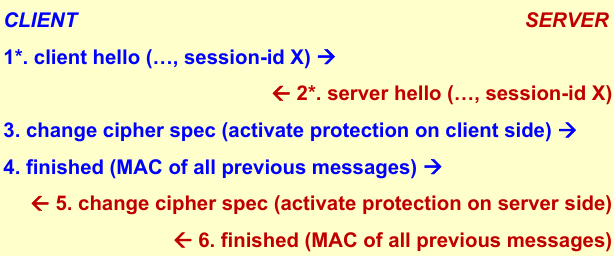
\includegraphics[width=.9\linewidth]{img/TLS resume session.png}
    \caption{TLS resume session.}
    \label{fig:tls-resume-session}
  \end{subfigure}
  \caption{TLS link teardown and resume session.}
\end{figure}

\section{TLS versions}
\subsection{TLS 1.0}
TLS 1.0, or SSL 3.1, was released in 1999. It is the first version of
the protocol, and it is based on SSL 3.0. Previous version were using
proprietary solutions, so the adoption of open standards was strongly
encouraged.

\subsection{TLS 1.1}
TLS 1.1 was released in 2006, and it introduced some security fixes
especially to protect against CBC attacks. In fact, the implicit
IV is replaced with an explicit IV to protect against CBC attacks.
Also protection against padding oracle attacks were introduces to
reduce the information leaks. For this reason Passing errors now use
the bad\_record\_mac alert message (rather than the decryption\_failed
one). Furthermore, premature closes no longer cause a session to be non-
resumable.

\subsection{TLS 1.2}
TLS 1.2 was released in 2008, and it introduced some new features and 
improvements. The chipersuite also specifies the pseudo random
function instead of leaving the choice to the implementation. The
sha-1 algorithm was replaced with SHA-256, and its also added support
for authenticated encryption, such as AES in GCN or CCM mode.

All the chipersuites tat use IDEA and DES are deprecated.

\section{TLS attacks}
\subsection{Heartbleed}
Heartbleed is a security bug in the OpenSSL cryptography library,
which is a widely used implementation of the TLS protocol. It was able
to exploit the fact that the heartbeat extension keeps the connection
alive without the need to negotiate the SSL session again. The
attacker could send a heartbeat request, but the length of the 
response is much longer( up to 64KB) than the actual data sent by the
client. This attack could then allow to leak memory contents.
